\documentclass[10pt]{article}
\usepackage[utf8]{inputenc}
\usepackage[T1]{fontenc}
\usepackage{amsmath}
\usepackage{amsfonts}
\usepackage{amssymb}
\usepackage[version=4]{mhchem}
\usepackage{stmaryrd}
\usepackage{graphicx}
\usepackage[export]{adjustbox}
\graphicspath{ {./images/} }

\title{JEE-MAIN EXAMINATION - APRIL 2025 \\
 (HELD ON TUESDAY \(\mathbf{0 8}^{\text {th }}\) APRIL 2025) \\
 TIME : 3:00 PM TO 6:00 PM }

\author{}
\date{}


\begin{document}
\maketitle
\section*{PHYSICS}
\section*{SECTION-A}
\begin{enumerate}
  \setcounter{enumi}{25}
  \item Given below are two statements: one is labelled as Assertion A and the other is labelled as Reason R Assertion A : Work done in moving a test charge between two points inside a uniformly charged spherical shell is zero, no matter which path is chosen.
\end{enumerate}

Reason R : Electrostatic potential inside a uniformly charged spherical shell is constant and is same as that on the surface of the shell.

In the light of the above statements, choose the correct answer from the options given below\\
(1) \(\mathbf{A}\) is true but \(\mathbf{R}\) is false\\
(2) Both \(\mathbf{A}\) and \(\mathbf{R}\) are true and \(\mathbf{R}\) is the correct explanation of \(\mathbf{A}\)\\
(3) \(\mathbf{A}\) is false but \(\mathbf{R}\) is true\\
(4) Both \(\mathbf{A}\) and \(\mathbf{R}\) are true but \(\mathbf{R}\) is NOT the correct explanation of \(\mathbf{A}\)

Ans. (2)\\
Sol. Conceptual\\
27. A rod of linear mass density ' \(\lambda\) ' and length ' \(L\) ' is bent to form a ring of radius ' R '. Moment of inertia of ring about any of its diameter is :\\
(1) \(\frac{\lambda L^{3}}{16 \pi^{2}}\)\\
(2) \(\frac{\lambda \mathrm{L}^{3}}{12}\)\\
(3) \(\frac{\lambda L^{3}}{4 \pi^{2}}\)\\
(4) \(\frac{\lambda L^{3}}{8 \pi^{2}}\)

Ans. (4)\\
Sol. \(\quad L=2 \pi R\)\\
\(\mathrm{I}=\frac{\mathrm{MR}^{2}}{2}=\frac{\lambda \times \mathrm{L}}{2} \times\left(\frac{\mathrm{L}}{2 \pi}\right)^{2}=\frac{\lambda \mathrm{L}^{3}}{8 \pi^{2}}\)

\section*{TEST PAPER WITH SOLUTION}
\begin{enumerate}
  \setcounter{enumi}{27}
  \item A 3 m long wire of radius 3 mm shows an extension of 0.1 mm when loaded vertically by a mass of 50 kg in an experiment to determine Young's modulus. The value of Young's modulus of the wire as per this experiment is \(\mathrm{P} \times 10^{11} \mathrm{Nm}^{-2}\), where the value of \(P\) is : (Take \(g=3 \pi \mathrm{~m} / \mathrm{s}^{2}\) )\\
(1) 5\\
(2) 10\\
(3) 25\\
(4) 2.5
\end{enumerate}

Ans. (1)\\
Sol. \(\frac{50 \mathrm{~g}}{\pi \mathrm{r}^{2}}=\mathrm{y} \cdot \frac{\Delta \ell}{\ell}\)\\
\(\frac{50 \times 3 \pi}{\pi \times\left(3 \times 10^{-3}\right)^{2}}=\mathrm{P} \times 10^{11} \times \frac{0.1 \times 10^{-3}}{3}\)\\
\(\Rightarrow \mathrm{P}=\frac{50 \times 3 \times 3}{3^{2} \times 10^{-6} \times 10^{11} \times 0.1 \times 10^{-3}}\)\\
\(\mathrm{P}=5\)\\
29. Electric charge is transferred to an irregular metallic disk as shown in figure. If \(\sigma_{1}, \sigma_{2}, \sigma_{3}\) and \(\sigma_{4}\) are charge densities at given points then, choose the correct answer from the options given below:\\
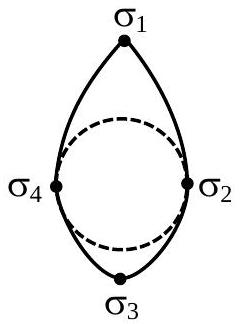
\includegraphics[max width=\textwidth, center]{2025_10_03_f92ebf7e4b400c69fbb6g-1}\\
(A) \(\sigma_{1}>\sigma_{3} ; \sigma_{2}=\sigma_{4}\)\\
(B) \(\sigma_{1}>\sigma_{2} ; \sigma_{3}>\sigma_{4}\)\\
(C) \(\sigma_{1}>\sigma_{3}>\sigma_{2}=\sigma_{4}\)\\
(D) \(\sigma_{1}<\sigma_{3}<\sigma_{2}=\sigma_{4}\)\\
(E) \(\sigma_{1}=\sigma_{2}=\sigma_{3}=\sigma_{4}\)\\
(1) A, B and C Only\\
(2) A and C Only\\
(3) D and E Only\\
(4) B and C Only

Ans. (1)\\
Sol. \(\sigma \propto \frac{1}{\mathrm{ROC}}\)\\
\((\mathrm{ROC})_{1}<(\mathrm{ROC})_{3}<(\mathrm{ROC})_{2}=(\mathrm{ROC})_{4}\)\\
\(\sigma_{1}>\sigma_{3}>\sigma_{2}=\sigma_{4}\)\\
30. Water falls from a height of 200 m into a pool. Calculate the rise in temperature of the water assuming no heat dissipation from the water in the pool.\\
\(\left(\right.\) Take \(\mathrm{g}=10 \mathrm{~m} / \mathrm{s}^{2}\), specific heat of water \(=4200 \mathrm{~J} /(\mathrm{kg} \mathrm{K})\) )\\
(1) 0.23 K\\
(2) 0.36 K\\
(3) 0.14 K\\
(4) 0.48 K

Ans. (4)\\
Sol. \(\mathrm{mgh}=\mathrm{ms} \Delta \mathrm{T}\)\\
\(\Delta \mathrm{T}=\frac{\mathrm{gh}}{\mathrm{s}}=\frac{10 \times 200}{4200} \mathrm{~K}=\frac{10}{21} \mathrm{~K}\)\\
31. A concave-convex lens of refractive index 1.5 and the radii of curvature of its surfaces are 30 cm and 20 cm , respectively. The concave surface is upwards and is filled with a liquid of refractive index 1.3. The focal length of the liquid-glass combination will be\\
(1) \(\frac{500}{11} \mathrm{~cm}\)\\
(2) \(\frac{800}{11} \mathrm{~cm}\)\\
(3) \(\frac{700}{11} \mathrm{~cm}\)\\
(4) \(\frac{600}{11} \mathrm{~cm}\)

Ans. (4)\\
Sol.\\
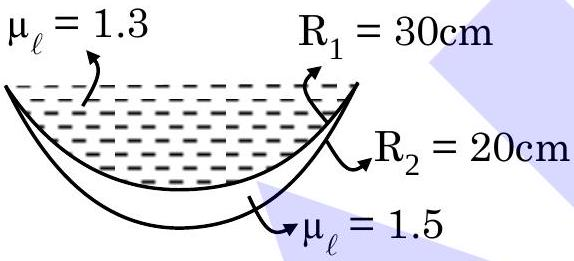
\includegraphics[max width=\textwidth, center]{2025_10_03_f92ebf7e4b400c69fbb6g-2(2)}

\[
\begin{aligned}
\frac{1}{\mathrm{f}} & =\left(\frac{1.3-1}{1}\right)\left(\frac{1}{\infty}-\frac{1}{-30}\right) \\
& =\left(\frac{1.5-1}{1}\right)\left(\frac{1}{-30}-\frac{1}{-30}\right) \\
& =\frac{0.3}{30}+\frac{0.5}{60}=\frac{1}{100}+\frac{1}{120} \\
& =\frac{6+5}{600}=\frac{11}{600} \\
\mathrm{f} & =\frac{600}{11} \mathrm{~cm}
\end{aligned}
\]

\begin{enumerate}
  \setcounter{enumi}{31}
  \item An infinitely long wire has uniform linear charge density \(\lambda=2 \mathrm{nC} / \mathrm{m}\). The net flux through a Gaussian cube of side length \(\sqrt{3} \mathrm{~cm}\), if the wire passes through any two corners of the cube, that are maximally displaced from each other, would be \(\mathrm{xNm}^{2} \mathrm{C}^{-1}\), where x is :\\[0pt]
[Neglect any edge effects and use \(\frac{1}{4 \pi \varepsilon_{0}}=9 \times 10^{9}\) SI units]\\
(1) \(0.72 \pi\)\\
(2) \(1.44 \pi\)\\
(3) \(6.48 \pi\)\\
(4) \(2.16 \pi\)
\end{enumerate}

Ans. (4)\\
Sol.\\
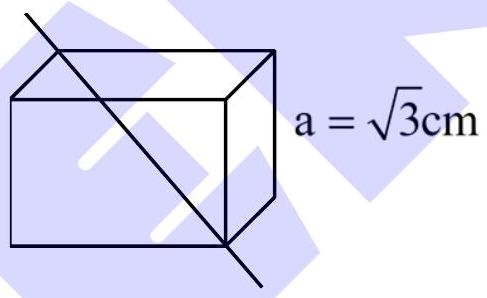
\includegraphics[max width=\textwidth, center]{2025_10_03_f92ebf7e4b400c69fbb6g-2(1)}\\
\(\phi=\frac{\mathrm{q}_{\text {enc }}}{\varepsilon_{0}}=\frac{\lambda \cdot \sqrt{3} \mathrm{a}}{\varepsilon_{0}}\)\\
\(=2 \times 10^{-9} \times \sqrt{3} \times \sqrt{3} \times 10^{-2} \times 36 \pi \times 10^{9} \mathrm{Nm}^{2} \mathrm{C}^{-1}\)\\
\(=2.16 \pi \mathrm{Nm}^{2} \mathrm{C}^{-1}\)\\
33. The output voltage in the following circuit is (Consider ideal diode case)\\
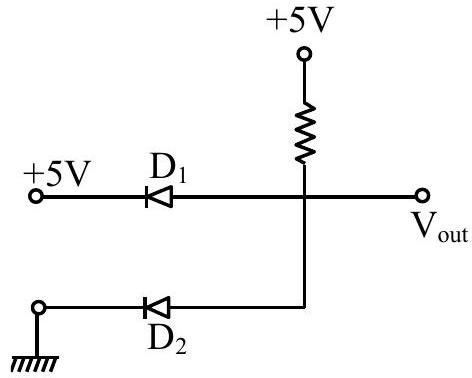
\includegraphics[max width=\textwidth, center]{2025_10_03_f92ebf7e4b400c69fbb6g-2}\\
(1) 10 V\\
(2) 0 V\\
(3) +5 V\\
(4) -5 V

Ans. (2)

Sol. Here \(\mathrm{D}_{1}\) is reverse biased and \(\mathrm{D}_{2}\) is forward biased. Therefore current flow through \(\mathrm{D}_{\mathrm{Q}}\) and 5 V drop on resistor.

So, \(\mathrm{V}_{\text {out }}=0\)\\
34. Two metal spheres of radius \(R\) and \(3 R\) have same surface charge density \(\sigma\). If they are brought in contact and then separated, the surface charge density on smaller and bigger sphere becomes \(\sigma_{1}\) and \(\sigma_{2}\), respectively. The ratio \(\frac{\sigma_{1}}{\sigma_{2}}\) is.\\
(1) \(\frac{1}{9}\)\\
(2) 9\\
(3) \(\frac{1}{3}\)\\
(4) 3

Ans. (4)\\
Sol. For conducting sphere, \(\mathrm{V}=\frac{\sigma \mathrm{r}}{\varepsilon_{0}}\)\\
After contact, \(\mathrm{V}_{1}=\mathrm{V}_{2}\)\\
\(\sigma_{1} \mathrm{r}_{1}=\sigma_{2} \mathrm{r}_{2}\)\\
\(\frac{\sigma_{1}}{\sigma_{2}}=\frac{\mathrm{r}_{2}}{\mathrm{r}_{1}}\)\\
\(\frac{\sigma_{1}}{\sigma_{2}}=3\)\\
35. A quantity \(Q\) is formulated as \(X^{-2} Y^{+\frac{3}{2}} Z^{-\frac{2}{5}} \cdot X, Y\) and \(Z\) are independent parameters which have fractional errors of \(0.1,0.2\) and 0.5 , respectively in measurement. The maximum fractional error of \(Q\) is\\
(1) 0.1\\
(2) 0.8\\
(3) 0.7\\
(4) 0.6

Ans. (3)\\
Sol. Fractional error \(=2 \frac{\Delta \mathrm{X}}{\mathrm{X}}+\frac{3}{2} \frac{\Delta \mathrm{Y}}{\mathrm{Y}}+\frac{2}{5} \frac{\Delta \mathrm{Z}}{\mathrm{Z}}\)\\
\(=2(0.1)+\frac{3}{2}(0.2)+\frac{2}{5}(0.5)\)\\
\(=0.2+0.3+0.2=0.7\)\\
36. A monoatomic gas having \(\gamma=\frac{5}{3}\) is stored in a thermally insulated container and the gas is suddenly compressed to \(\left(\frac{1}{8}\right)^{\text {th }}\) of its initial volume. The ratio of final pressure and initial pressure is: ( \(\gamma\) is the ratio of specific heats of the gas at constant pressure and at constant volume)\\
(1) 16\\
(2) 40\\
(3) 32\\
(4) 28

Ans. (3)\\
Sol. \(\quad P_{i} V_{i}^{\gamma}=P_{f} V_{f}^{\gamma}\)\\
\(\frac{P_{f}}{P_{i}}=\left(\frac{V_{i}}{V_{f}}\right)^{\gamma}=(8)^{5 / 3}\)\\
\(\frac{\mathrm{P}_{\mathrm{f}}}{\mathrm{P}_{\mathrm{i}}}=32\)\\
37. A convex lens of focal length 30 cm is placed in contact with a concave lens of focal length 20 cm . An object is placed at 20 cm to the left of this lens system. The distance of the image from the lens in cm is \(\_\_\_\_\)\\
(1) 30\\
(2) 45\\
(3) \(\frac{60}{7}\)\\
(4) 15

Ans. (4)\\
Sol. Equivalent focal length\\
\(\frac{1}{\mathrm{f}}=\frac{1}{\mathrm{f}_{1}}+\frac{1}{\mathrm{f}_{2}}\)\\
\(=\frac{1}{30}+\frac{1}{-20}=\frac{2-3}{60}=-\frac{1}{60}\)\\
\(\mathrm{f}=-60 \mathrm{~cm}\)\\
Lens formula\\
\(\frac{1}{v}-\frac{1}{u}=\frac{1}{f}\)\\
\(\frac{1}{v}-\frac{1}{-20}=\frac{1}{-60}\)\\
\(\mathrm{v}=-15 \mathrm{~cm}\)\\
38. Two strings with circular cross section and made of same material, are stretched to have same amount of tension. A transverse wave is then made to pass through both the strings. The velocity of the wave in the first string having the radius of cross section R is \(\mathrm{v}_{1}\), and that in the other string having radius of cross section \(\mathrm{R} / 2\) is \(\mathrm{v}_{2}\). Then \(\frac{\mathrm{v}_{2}}{\mathrm{v}_{1}}=\)\\
(1) \(\sqrt{2}\)\\
(2) 2\\
(3) 8\\
(4) 4

Ans. (2)\\
Sol. \(v=\sqrt{\frac{T}{\mu}}=\sqrt{\frac{T}{f \pi R^{2}}}\)\\
\(\frac{\mathrm{v}_{2}}{\mathrm{v}_{1}}=\frac{\mathrm{R}_{1}}{\mathrm{R}_{2}}=2\)\\
39. Figure shows a current carrying square loop ABCD of edge length is ' \(a\) ' lying in a plane. If the resistance of the ABC part is r and that of ADC part is 2 r , then the magnitude of the resultant magnetic field at centre of the square loop is\\
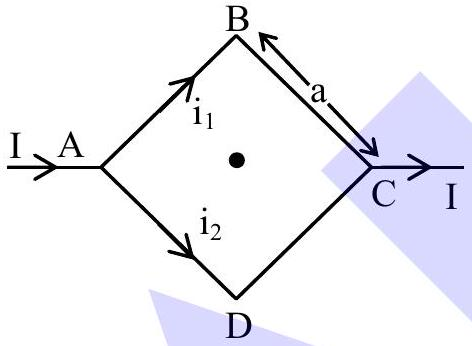
\includegraphics[max width=\textwidth, center]{2025_10_03_f92ebf7e4b400c69fbb6g-4(1)}\\
(1) \(\frac{3 \pi \mu_{0} I}{\sqrt{2} a}\)\\
(2) \(\frac{\mu_{0} I}{2 \pi a}\)\\
(3) \(\frac{\sqrt{2} \mu_{o} I}{3 \pi a}\)\\
(4) \(\frac{2 \mu_{0} I}{3 \pi a}\)

Ans. (3)

Sol.\\
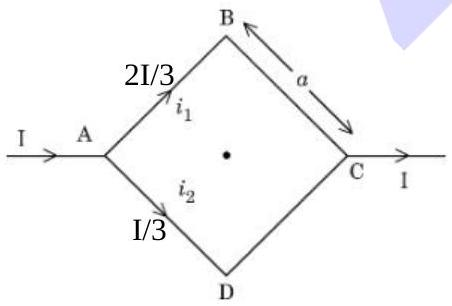
\includegraphics[max width=\textwidth, center]{2025_10_03_f92ebf7e4b400c69fbb6g-4}\\
\(\overrightarrow{\mathrm{B}}=\overrightarrow{\mathrm{B}}_{\mathrm{AB}}+\overrightarrow{\mathrm{B}}_{\mathrm{BC}}+\overrightarrow{\mathrm{B}}_{\mathrm{CD}}+\overrightarrow{\mathrm{B}}_{\mathrm{DA}}\)\\
\(\overrightarrow{\mathrm{B}}=\left[\frac{-\mu_{0}(2 \mathrm{I} / 3)}{4 \pi(\mathrm{a} / 2)} \sqrt{2}-\frac{\mu_{0}(2 \mathrm{I} / 3)}{4 \pi(\mathrm{a} / 2)} \sqrt{2}\right.\)

\[
\left.+\frac{\mu_{0}(I / 3)}{4 \pi(a / 2)} \sqrt{2}+\frac{\mu_{0}(I / 3)}{4 \pi(a / 2)} \sqrt{2}\right] \hat{k}
\]

\(\overrightarrow{\mathrm{B}}=\left[\frac{-2 \sqrt{2} \mu_{0} \mathrm{I}}{3 \pi \mathrm{a}}+\frac{\sqrt{2} \mu_{0} \mathrm{I}}{3 \pi \mathrm{a}}\right] \hat{\mathrm{k}}\)\\
\(\vec{B}=\frac{-\sqrt{2} \mu_{0} I}{3 \pi a} \hat{k}\)\\
40. A body of mass 2 kg moving with velocity of \(\overrightarrow{\mathrm{v}}_{\text {in }}=3 \hat{\mathrm{i}}+4 \hat{\mathrm{j}} \mathrm{ms}^{-1}\) enters into a constant force field of 6 N directed along positive \(z\)-axis. If the body remains in the field for a period of \(\frac{5}{3}\) seconds, then velocity of the body when it emerges from force field is\\
(1) \(4 \hat{i}+3 \hat{j}+5 \hat{k}\)\\
(2) \(3 \hat{i}+4 \hat{j}+5 \hat{k}\)\\
(3) \(3 \hat{i}+4 \hat{j}-5 \hat{k}\)\\
(4) \(3 \hat{i}+4 \hat{j}+\sqrt{5} \hat{k}\)

Ans. (2)\\
Sol. \(\quad \vec{a}=\frac{B}{2} \hat{k}=3 \hat{k}, t=\frac{5}{3} s\)

\[
\begin{aligned}
& \overrightarrow{\mathrm{u}}=3 \hat{\mathrm{i}}+4 \hat{\mathrm{j}} \\
& \overrightarrow{\mathrm{v}}=\overrightarrow{\mathrm{u}}+\overrightarrow{\mathrm{at}}=3 \hat{\mathrm{i}}+4 \hat{\mathrm{j}}+5 \hat{\mathrm{k}}
\end{aligned}
\]

\begin{enumerate}
  \setcounter{enumi}{40}
  \item Two balls with same mass and initial velocity, are projected at different angles in such a way that maximum height reached by first ball is 8 times higher than that of the second ball. \(\mathrm{T}_{1}\) and \(\mathrm{T}_{2}\) are the total flying times of first and second ball, respectively, then the ratio of \(T_{1}\) and \(T_{2}\) is :\\
(1) \(2 \sqrt{2}: 1\)\\
(2) \(2: 1\)\\
(3) \(\sqrt{2}: 1\)\\
(4) \(4: 1\)
\end{enumerate}

Ans. (1)

\section*{Level up your prep for JEE with ALLEN Online's LIVE JEE course!}
Sol. Given, \(\left(\mathrm{H}_{\text {max }}\right)_{1}=8 \times\left(\mathrm{H}_{\text {max }}\right)_{2}\)\\
\(\frac{\mathrm{u}^{2} \sin ^{2} \theta_{1}}{2 \mathrm{~g}}=8 \times \frac{\mathrm{u}^{2} \sin ^{2} \theta_{2}}{2 \mathrm{~g}}\)\\
\(\Rightarrow \sin \theta_{1}=2 \sqrt{2} \sin \theta_{2}\)\\
\(\frac{\mathrm{T}_{1}}{\mathrm{~T}_{2}}=\frac{2 \mathrm{u} \sin \theta_{1} / \mathrm{g}}{2 \mathrm{u} \sin \theta_{2} / \mathrm{g}}=\frac{\sin \theta_{1}}{\sin \theta_{2}}=2 \sqrt{2}\)\\
42. The amplitude and phase of a wave that is formed by the superposition of two harmonic travelling waves, \(\mathrm{y}_{1}(\mathrm{x}, \mathrm{t})=4 \sin (\mathrm{kx}-\omega \mathrm{t})\) and\\
\(\mathrm{y}_{2}(\mathrm{x}, \mathrm{t})=2 \sin \left(\mathrm{kx}-\omega \mathrm{t}+\frac{2 \pi}{3}\right)\), are \(:\)\\
(Take the angular frequency of initial waves same as \(\omega\) )\\
(1) \(\left[6, \frac{2 \pi}{3}\right]\)\\
(2) \(\left[6, \frac{\pi}{3}\right]\)\\
(3) \(\left[\sqrt{3}, \frac{\pi}{6}\right]\)\\
(4) \(\left[2 \sqrt{3}, \frac{\pi}{6}\right]\)

Ans. (4)\\
Sol.\\
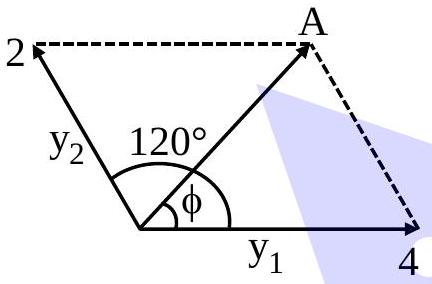
\includegraphics[max width=\textwidth, center]{2025_10_03_f92ebf7e4b400c69fbb6g-5}

\[
\begin{aligned}
\mathrm{A} & =\sqrt{2^{2}+4^{2}+2 \times 2 \times 4 \times \cos 120^{\circ}} \\
& =\sqrt{12}=2 \sqrt{3}
\end{aligned}
\]

\(\tan \phi=\frac{2 \sin 120^{\circ}}{4+2 \cos 120^{\circ}}=\frac{\sqrt{3}}{3}=\frac{1}{\sqrt{3}}\)\\
\(\phi=\frac{\pi}{6}\)\\
43. In a Young's double slit experiment, the source is white light. One of the slits is covered by red filter and another by a green filter. In this case\\
(1) There shall be an interference pattern for red distinct from that for green.\\
(2) There shall be no interference fringes.\\
(3) There shall be alternate interference fringes of red and green.\\
(4) There shall be an interference pattern, where each fringe's pattern center is green and outer edges is red.

Ans. (2)\\
Sol. Different colours will have different fringe width. Within a few fringes of red, there will be several fringes of violet.\\
Also, there will be overlapping of colours.\\
44. For a nucleus of mass number A and radius R , the mass density of nucleus can be represented as\\
(1) \(\mathrm{A}^{3}\)\\
(2) \(\mathrm{A}^{\frac{1}{3}}\)\\
(3) \(\mathrm{A}^{\frac{2}{3}}\)\\
(4) Independent of A

Ans. (4)\\
Sol. Conceptual\\
45. A block of mass 2 kg is attached to one end of a massless spring whose other end is fixed at a wall. The spring-mass system moves on a frictionless horizontal table. The spring's natural length is 2 m and spring constant is \(200 \mathrm{~N} / \mathrm{m}\). The block is pushed such that the length of the spring becomes 1 m and then released. At distance \(\mathrm{x} \mathrm{m}(\mathrm{x}<2)\) from the wall. the speed of the block will be :\\
(1) \(10[1-(2-\mathrm{x})]^{3 / 2} \mathrm{~m} / \mathrm{s}\)\\
(2) \(10\left[1-(2-x)^{2}\right]^{1 / 2} \mathrm{~m} / \mathrm{s}\)\\
(3) \(10\left[1-(2-x)^{2}\right] \mathrm{m} / \mathrm{s}\)\\
(4) \(10\left[1-(2-\mathrm{x})^{2}\right]^{2} \mathrm{~m} / \mathrm{s}\)

Ans. (2)

Sol.\\
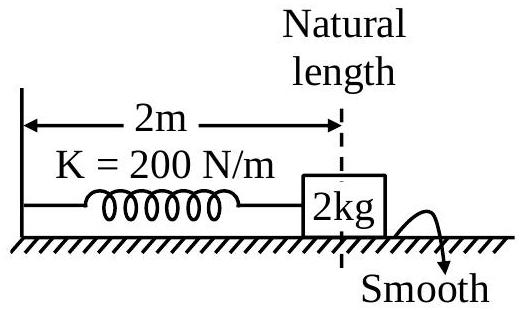
\includegraphics[max width=\textwidth, center]{2025_10_03_f92ebf7e4b400c69fbb6g-6}

Given, Natural length of spring \(=2 \mathrm{~m}\)\\
Initial compression in spring \(\left(\mathrm{x}_{\mathrm{i}}\right)=1 \mathrm{~m}\)\\
Final compression in spring \(\left(\mathrm{x}_{\mathrm{f}}\right)=(2-\mathrm{x}) \mathrm{m}\)\\
Using energy conservation\\
\(\mathrm{K}_{\mathrm{i}}+\mathrm{U}_{\mathrm{i}}=\mathrm{K}_{\mathrm{f}}+\mathrm{U}_{\mathrm{f}}\)\\
\(0+\frac{1}{2} K x_{i}^{2}=\frac{1}{2} m v^{2}+\frac{1}{2} K x_{f}^{2}\)\\
\(\frac{1}{2} m v^{2}=\frac{1}{2} K\left(x_{i}^{2}-x_{f}^{2}\right)\)\\
\(\frac{1}{2} \times 2 \times \mathrm{v}^{2}=\frac{1}{2} \times 200 \times\left(1^{2}-(2-\mathrm{x})^{2}\right)\)\\
\(\mathrm{v}^{2}=100\left[1-(2-\mathrm{x})^{2}\right]\)\\
\(\mathrm{v}=10\left[1-(2-\mathrm{x})^{2}\right]^{1 / 2}\)

\section*{SECTION-B}
\begin{enumerate}
  \setcounter{enumi}{45}
  \item An electron is released from rest near an infinite non-conducting sheet of uniform charge density \('-\sigma\) '. The rate of change of de-Broglie wave length associated with the electron varies inversely as \(\mathrm{n}^{\text {th }}\) power of time. The numerical value of \(n\) is \(\_\_\_\_\) .\\
Ans. (2)\\
Sol. Let the momentum of \(\mathrm{e}^{-}\)at any time t is p and its de-broglie wavelength is \(\lambda\).\\
Then, \(\mathrm{p}=\frac{\mathrm{h}}{\lambda}\)\\
\(\frac{\mathrm{dp}}{\mathrm{dt}}=\frac{-\mathrm{h}}{\lambda^{2}} \frac{\mathrm{~d} \lambda}{\mathrm{dt}}\)\\
\(\mathrm{ma}=\mathrm{F}=-\frac{\mathrm{h}}{\lambda} \frac{\mathrm{d} \lambda}{\mathrm{dt}} \quad\left[\mathrm{m}=\right.\) mass of \(\left.\mathrm{e}^{-}\right]\)\\
Where, -ve sign represents decrease in \(\lambda\) with time \(\mathrm{ma}=\frac{-\mathrm{h}}{(\mathrm{h} / \mathrm{p})^{2}} \frac{\mathrm{~d} \lambda}{\mathrm{dt}}\)\\
\(\mathrm{a}=-\frac{\mathrm{p}^{2}}{\mathrm{mh}} \frac{\mathrm{d} \lambda}{\mathrm{dt}}\)\\
\(a=-\frac{m v^{2}}{h} \frac{d \lambda}{d t}\)\\
\(\frac{\mathrm{d} \lambda}{\mathrm{dt}}=-\frac{\mathrm{ah}}{\mathrm{mv}^{2}}\)\\
here, \(\mathrm{a}=\frac{\mathrm{qE}}{\mathrm{m}}=\frac{\mathrm{e}}{\mathrm{m}} \frac{\sigma}{2 \varepsilon_{0}}\)\\
\(\mathrm{a}=\frac{\sigma \mathrm{e}}{2 \mathrm{~m} \varepsilon_{0}}\)\\
and \(\mathrm{v}=\mathrm{u}+\) at\\
\(\mathrm{v}=\mathrm{at}\)\\
Substituting values of \(\mathrm{a} \& \mathrm{v}\) in equation (1)\\
\(\frac{\mathrm{d} \lambda}{\mathrm{dt}}=-\frac{2 \mathrm{~h} \varepsilon_{0}}{\sigma \mathrm{et}^{2}}\)\\
\(\Rightarrow \frac{\mathrm{d} \lambda}{\mathrm{dt}} \propto \frac{1}{\mathrm{t}^{2}}\)\\
\(\Rightarrow \mathrm{n}=2\)
  \item A sample of a liquid is kept at 1 atm . It is compressed to 5 atm which leads to change of volume of \(0.8 \mathrm{~cm}^{3}\). If the bulk modulus of the liquid is 2 GPa , the initial volume of the liquid was\\
\(\_\_\_\_\) litre. (Take \(1 \mathrm{~atm}=10^{5} \mathrm{~Pa}\) )\\
Ans. (4)\\
Sol. Given, Initial pressure of liquid \(\left(\mathrm{P}_{\mathrm{i}}\right)=1 \mathrm{~atm}\)\\
Final pressure of liquid \(\left(\mathrm{P}_{\mathrm{f}}\right)=5 \mathrm{~atm}\)\\
Change in pressure \((\mathrm{dP})=\mathrm{P}_{\mathrm{f}}-\mathrm{P}_{\mathrm{i}}=4 \mathrm{~atm}\)\\
\(=4 \times 10^{5} \mathrm{~Pa}\)\\
Change in volume \((\mathrm{dV})=-0.8 \mathrm{~cm}^{3}\)\\
Bulk modulus \((\mathrm{B})=2 \times 10^{9} \mathrm{~Pa}\)\\
Now, \(B=\frac{-d P}{(d V / V)} \Rightarrow V=-B\left(\frac{d V}{d P}\right)\)\\
\(\Rightarrow \mathrm{V}=-2 \times 10^{9} \times \frac{\left(-0.8 \times 10^{-6}\right)}{4 \times 10^{5}}\)\\
\(=4 \times 10^{-3} \mathrm{~m}^{3}=4\) litre
\end{enumerate}

\section*{Level up your prep for JEE with ALLEN Online's LIVE JEE course!}
48.

\begin{center}
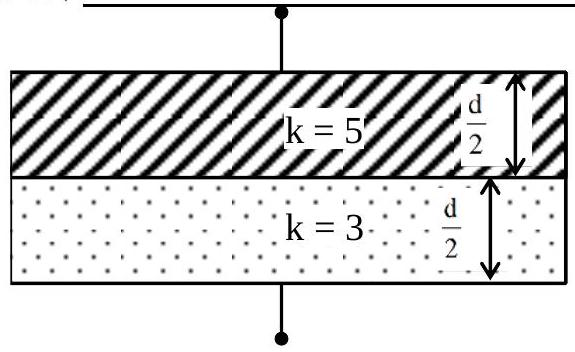
\includegraphics[max width=\textwidth]{2025_10_03_f92ebf7e4b400c69fbb6g-7(2)}
\end{center}

Space between the plates of a parallel plate capacitor of plate area \(4 \mathrm{~cm}^{2}\) and separation of (d) 1.77 mm , is filled with uniform dielectric materials with dielectric constants ( 3 and 5 ) as shown in figure. Another capacitor of capacitance 7.5 pF is connected in parallel with it. The effective capacitance of this combination is \(\_\_\_\_\) pF .\\
(Given \(\varepsilon_{0}=8.85 \times 10^{-12} \mathrm{~F} / \mathrm{m}\) )\\
Ans. (15)\\
Sol.\\
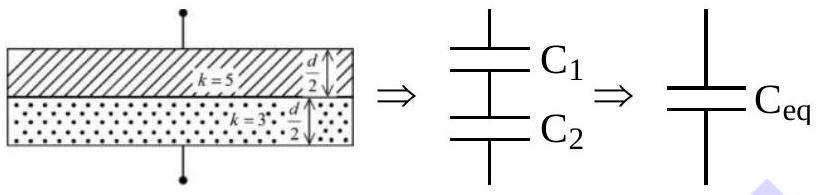
\includegraphics[max width=\textwidth, center]{2025_10_03_f92ebf7e4b400c69fbb6g-7(1)}\\
\(\mathrm{C}_{1}=\frac{5 \times 4 \times 10^{-4} \times 8.85 \times 10^{-12}}{\frac{1.77}{2} \times 10^{-3}}=20 \mathrm{pF}\)\\
\(\mathrm{C}_{2}=\frac{3 \times 4 \times 10^{-4} \times 8.85 \times 10^{-12}}{\frac{1.77}{2} \times 10^{-3}}=12 \mathrm{pF}\)\\
\(\mathrm{C}_{\mathrm{eq}}=\frac{\mathrm{C}_{1} \mathrm{C}_{2}}{\mathrm{C}_{1}+\mathrm{C}_{2}}=\frac{12 \times 20}{12+20}=7.5 \mathrm{pF}\)\\
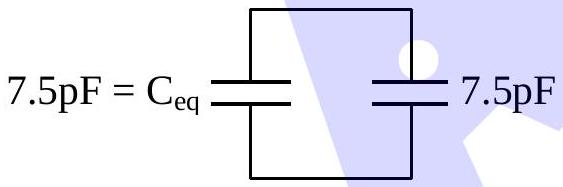
\includegraphics[max width=\textwidth, center]{2025_10_03_f92ebf7e4b400c69fbb6g-7}

Finally equivalent capacitance\\
\(\left(\mathrm{C}_{\text {eq }}\right)_{\text {final }}=7.5+7.5=15 \mathrm{pF}\)\\
49. A thin solid disk of 1 kg is rotating along its diameter axis at the speed of 1800 rpm . By applying an external torque of \(25 \pi \mathrm{Nm}\) for 40 s , the speed increases to 2100 rpm . The diameter of the disk is \(\_\_\_\_\) m.

Sol. Given, \(\mathrm{m}=1 \mathrm{~kg}\)\\
\(\omega_{\mathrm{i}}=1800 \mathrm{rpm}=1800 \times \frac{2 \pi}{60}=60 \pi \frac{\mathrm{rad}}{\mathrm{sec}}\)\\
\(\omega_{\mathrm{f}}=2100 \mathrm{rpm}=2100 \times \frac{2 \pi}{60}=70 \pi \frac{\mathrm{rad}}{\mathrm{sec}}\)\\
\(\tau_{\text {ext }}=25 \pi \mathrm{Nm}\)\\
\(\mathrm{t}=40 \mathrm{sec}\)\\
Using equation of motion\\
\(\omega_{\mathrm{f}}=\omega_{\mathrm{i}}+\alpha \mathrm{t}\)\\
\(70 \pi=60 \pi+\alpha(40)\)\\
\(\alpha=\frac{\pi}{4} \mathrm{rad} / \mathrm{sec}^{2}\)\\
Also, \(\tau=\mathrm{I} \alpha\)\\
\(\tau=\frac{m R^{2}}{4} \alpha\)\\
\(25 \pi=\frac{1 \times \mathrm{R}^{2}}{4} \times \frac{\pi}{4}\)\\
\(\mathrm{R}=20 \mathrm{~m}\)\\
Hence, diameter of disk \(=2 \mathrm{R}=2 \times 20=40 \mathrm{~m}\)\\
50. A cube having a side of 10 cm with unknown mass and 200 gm mass were hung at two ends of an uniform rigid rod of 27 cm long. The rod along with masses was placed on a wedge keeping the distance between wedge point and 200 gm weight as 25 cm . Initially the masses were not at balance. A beaker is placed beneath the unknown mass and water is added slowly to it. At given point the masses were in balance and half volume of the unknown mass was inside the water.\\
(Take the density of unknown mass is more than that of the water, the mass did not absorb water and water density is \(1 \mathrm{gm} / \mathrm{cm}^{3}\).) The unknown mass is \(\_\_\_\_\) kg.

Ans. (3)

Sol.\\
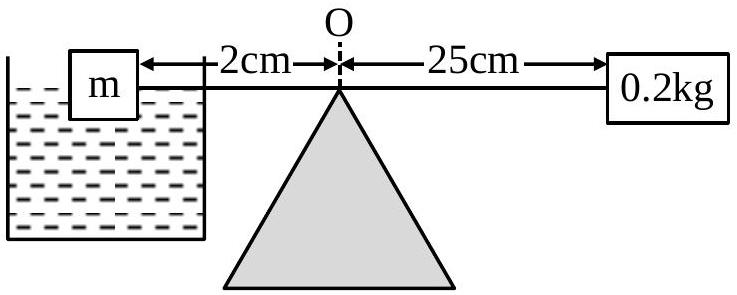
\includegraphics[max width=\textwidth, center]{2025_10_03_f92ebf7e4b400c69fbb6g-8(2)}

Given, volume of block \(=\left(10 \times 10^{-2}\right)^{3}=10^{-3} \mathrm{~m}^{3}\)\\
Let density of block \(=\rho \mathrm{kg} / \mathrm{m}^{3}\)\\
mass of block \(=\rho \times 10^{-3} \mathrm{~kg}\)\\
Buoyant Force \(\left(\mathrm{F}_{\mathrm{B}}\right)=1000 \times \frac{10^{-3}}{2} \times 10=5 \mathrm{~N}\)\\
F.B.D. of blocks\\
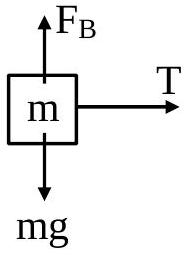
\includegraphics[max width=\textwidth, center]{2025_10_03_f92ebf7e4b400c69fbb6g-8}\\
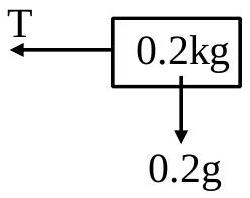
\includegraphics[max width=\textwidth, center]{2025_10_03_f92ebf7e4b400c69fbb6g-8(1)}

Balancing torque about point O , we get\\
\(\operatorname{mg}\left(2 \times 10^{-2}\right)-\mathrm{F}_{\mathrm{B}}\left(2 \times 10^{-2}\right)=0.2 \mathrm{~g}\left(25 \times 10^{-2}\right)\)\\
\(\rho \times 10^{-3} \times 10 \times 2-10=50\)\\
\(\rho=3000 \mathrm{~kg} / \mathrm{m}^{3}\)\\
Hence, mass of block \(=\rho \times 10^{-3}\)\\
\(=3000 \times 10^{-3}=3 \mathrm{~kg}\)

\section*{Level up your prep for JEE with our LIVE JEE Courses!}
LIVE classes with top Kota faculty\\
ALLEN's study material\\
Tests with national benchmarking\\
ALLEN App Advantage: 24/7 doubt support, Custom Practice \& more

Enrol Now

\section*{ALLEN ONLINE}
\section*{Secure up to}
\section*{90\% scholarship on our Online Courses!}
\section*{based on your JEE Main 2025 scores!}
Enrol Now


\end{document}